\section{Introduction}
Work presented in previous chapters highlighted the much improved \textit{ab initio} decoy quality achievable by restraining the conformational search space with residue-residue contact information. Furthermore, the data also highlighted that this improvement extends AMPLE's performance of achieving structure solution for more challenging targets. However, the data also indicated that AMPLE's current protocol is not tailored towards decoy sets with overall much higher accuracy. In some cases, decoy sets with correctly predicted folds --- whereby the mean \gls{tmscore} of the decoy set is greater than 0.5 score units --- did not generate any successful ensemble search models. It also became apparent that certain decoy sets contained some very high-quality decoys, but that these were often lost in the process of clustering due to the lack of other similar predictions.

Furthermore, \textit{ab initio} decoy similarity to the crystal structure was exceptionally high in some cases (\gls{rmsd} $<1.5$\AA). Although challenging by current means to identify these decoys, it is of great interest to structural biologists to do so since these decoys might be sufficient by themselves as \gls{mr} search models. Contact information, which is typically used to restrain the folding protocol might provide enough information to drive such identification. Indeed, \textcite{Kosciolek2014-bt} and \textcite{De_Oliveira2017-gj} highlighted the usefulness of long-range residue-residue contact pair satisfaction for model selection since it correlates well with decoy quality. Additionally, \textcite{Adhikari2018-lj} use long-range contact satisfaction routinely in CONFOLD2 to exclude the worst decoys amongst the set predicted ones.

Thus, this chapter focuses on exploring alternative strategies of decoy selection in AMPLE. In particular, work presented here focuses on exploiting long-range contact information to drive search model generation to extend AMPLE's performance on difficult cases further.

\section{Materials \& Methods}
\subsection{Target selection}
The dataset for this study consisted of 113 ROSETTA decoy sets generated throughout the work outlined in previous chapters. The 113 decoy sets covered all targets in the ORIGINAL (\cref{table:appendix_dataset_original}), PREDICTORS (\cref{table:appendix_dataset_predictors}) and TRANSMEMBRANE (\cref{table:appendix_dataset_transmembrane}) datasets. Top-$L$ ($>5$ residues sequence separation) CCMPRED \cite{Seemayer2014-zp}, PCONSC2 \cite{Skwark2014-qp}, METAPSICOV STAGE 1 \cite{Jones2015-vq} and MEMBRAIN \cite{Yang2013-bf} contact pairs were used in combination with the \textit{FADE} energy function to restrain the \textit{ab initio} structure prediction process.

\subsection{Computation of range-specific satisfaction scores}
The satisfaction of short- ($>5$ residues sequence separation), medium- ($>12$ residues sequence separation) and long-range contact pairs ($>23$ residues sequence separation; see \cref{sec:methods_longrange_satisfaction}) were computed for each decoy in each set. Hereby, the short-, medium- or long-range predicted contacts were extracted from the original predictions used to restrain the \textit{ab initio} structure prediction, matched against the contact pairs observed in individual decoys and the range-specific contact satisfaction score evaluated. 

\subsection{Decoy subselection} \label{sec:ample_decoys_decoy_selection}
Each set of decoys was ranked in descending order by their long-range contact pair satisfaction scores and the $n$ decoys with the lowest scores removed from each set. The number of decoys to remove $n$ was selected using a number of different strategies:

\begin{description}[style=multiline,leftmargin=4cm]
    \item[\textit{NONE}] leave the original set unchanged
    \item[\textit{LINEAR}] remove the worst 500 decoys
    \item[\textit{CUTOFF}] remove all decoys with a score of $<0.287$ 
    \item[\textit{SCALED}] remove all decoys with a scaled score of $<0.5$, where the scaled score is score divided by set average
    \item[\textit{INDIVIDUAL}] keep the top-5 decoys only
\end{description}

The fixed definition in the \textit{CUTOFF} strategy was determined by \textcite{De_Oliveira2017-gj}. The scaled score used by the \textit{SCALED} strategy was computed by dividing each decoy's long-range contact pair satisfaction by the set's average.

The \textit{INDIVIDUAL} subselection strategy differs substantially from the others. The top-5 decoys by long-range contact satisfaction were selected and subjected to treatment outside of AMPLE. The per-decoy treatments were the following:

\begin{description}[style=multiline,leftmargin=4cm]
    \item[default] leave the decoy unchanged
    \item[domain] remove all residues with $kde<\frac{1}{2}max_{kde}$, where $kde$ corresponds to the \gls{kde} and $max_{kde}$ to the maximum \gls{kde} obtained by applying the algorithm described by \textcite{Sadowski2013-zu} to the top-5$L$ contact map
    \item[dssp] remove all residues with secondary structure of ``helix turn (T)'', ``bend (S)'' or ``coil (C)'', which were assigned using DSSP \cite{Frishman1995-si} 
    \item[fragment] remove all residues that do not satisfy the following condition: extract all contacts from a decoy [C\textbeta\ distance of $<8$\AA\ (C\textalpha\ in case of Gly)] and reconstruct the decoy's sequence using the residue indices present in the set of contacts, then keep residues that are within a sequence fragment of at least three consecutive residues
    \item[variance] remove all residues with variance of more than 5\AA\textsuperscript{2}, which was extracted from the decoy's corresponding cluster in the \textit{NONE} subselection strategy
\end{description}

\subsection{Molecular Replacement} \label{subsec:ample_decoys_methods_mr}
To evaluate the benefits of such subselection to \gls{mr} in AMPLE, a subset of 35 decoy sets (spanning 35 unique targets) were processed as described above and subjected to AMPLE v1.2.0 and CCP4 v7.0.28. Default options were chosen with the following exceptions: decoys in all 10 clusters were used, subcluster radii thresholds were set to 1 and 3\AA, and side-chain treatments were set to \texttt{polyala} only. This change in protocol from AMPLE's initial mode of operation \cite{Bibby2012-lm} was shown to be advantageous in most cases by \textcite{Thomas2017-qu}, and thus trialled in this context. 

To allow comparability of these results to previous AMPLE runs, an additional condition was added, namely \textit{NONE\_classic}. The decoy set from the \textit{NONE} strategy was thereby subjected to the AMPLE protocol with default settings except \texttt{-num\_clusters}, which was set to sample the three largest clusters. Thus, the \textit{NONE\_classic} strategy differed from the \textit{NONE} one in three spects: top-3 clusters are used instead of top-10, 1, 2 and 3\AA\ subclustering radii are used instead of 1 and 3\AA\ only, and the most-reliable and all-atom side-chain treatments are kept.

All individual decoys created under the \textit{INDIVIDUAL} strategy were subjected as poly-Alanine decoys to MRBUMP \cite{Keegan2018-kn} with identical settings to those used in AMPLE. 

Each \gls{mr} run was assessed using the criteria defined in \cref{sec:methods_mr_success}.

\section{Results}
This chapter focuses on identifying further uses of predicted residue-residue contact pairs in unconventional \gls{mr}. In particular, the exclusion of \textit{ab initio} decoys by their contact satisfaction scores was investigated. A total of 113 decoy datasets were used to identify potential means of identifying the best or worst decoys. Furthermore, three strategies were trialled alongside two standard approaches to test the consequences of excluding the worst decoys in ensemble search model preparation in AMPLE.

\subsection{Contact pair satisfaction correlates with decoy quality}
\textcite{Kosciolek2014-bt} previously identified a correlation between the TM-score of a decoy and its fraction of satisfied contact pairs. Although reporting striking positive correlations (short-range:$\rho=0.50$; medium-range:$\rho=0.57$; long-range: $\rho=0.87$) for top-1 decoys, the study by \textcite{Kosciolek2014-bt} was limited to 10 representative targets with a maximum chain length of 158 residues. Furthermore, FRAGFOLD \cite{Jones2001-mc} was used for \textit{ab initio} protein structure prediction, a method with inferior performance to ROSETTA \cite{Rohl2004-dj} when using the decoys in unconventional \gls{mr} (see \cref{chap:alternate_abinitio_protocols}). Thus, the more diverse set of decoys generated in this study might be more representative in determining a correlation between decoy TM-scores and contact pair satisfaction.

A Pearson's \gls{cc} analysis with 113 ROSETTA decoy sets representing 56 globular and transmembrane targets shows a positive linear correlations between a decoy's TM-score and short-, medium- and long-range contact satisfaction (\cref{table:ample_decoys_tmscore_consat}). Furthermore, separating the correlation analysis of all targets by fold classification reveals that all-\textalpha, mixed \textalpha-\textbeta\ and transmembrane protein targets show the strongest positive correlations for long-range contact satisfaction (\cref{table:ample_decoys_tmscore_consat}). All-\textbeta\ and mixed \textalpha-\textbeta\ decoy sets show the strongest correlations for short- and medium-range contact satisfaction, whereby the former shows a stronger positive correlation between the decoy's TM-score and its medium-range contact satisfaction than its long-range contact satisfaction (medium-range:$\rho=0.54$; long-range:$\rho=0.50$) (\cref{table:ample_decoys_tmscore_consat}). Notably, the decoys of transmembrane protein targets show no significant correlation between TM-score and short-range contact satisfaction ($\rho=0.08$; \cref{table:ample_decoys_tmscore_consat}).

\begin{table}[H]
  \centering
  \caption[Correlation analysis between decoy TM-score and contact satisfaction]{Pearson's \gls{cc} analysis between a ROSETTA decoy's TM-score and short-, medium- and long-range contact satisfaction. Probability values for all $\rho$ coefficients is $<0.01$.}
  \label{table:ample_decoys_tmscore_consat}
  \begin{tabularx}{\textwidth}{X X X X}
      \hline
      \multirow{2}{*}{\textbf{Target class}} & \multicolumn{3}{c}{\textbf{Pearson's \gls{cc}}} \\ \cline{2-4}
      & Short-range   & Medium-range  & Long-range \\
      \hline
      all                               & 0.11          & 0.18          & 0.64 \\
      all-\textalpha                    & 0.30          & 0.44          & 0.69 \\
      all-\textbeta                     & 0.40          & 0.54          & 0.50 \\
      mixed \textalpha-\textbeta        & 0.42          & 0.55          & 0.69 \\
      transmembrane                     & 0.08          & 0.48          & 0.70 \\
      \hline
  \end{tabularx}
\end{table}

Following on from the Pearson's \gls{cc} analysis, a linear regression model was fitted to individual subsets of the data used for the correlation analysis to see if a decoy's TM-score could be predicted from its contact satisfaction score. However, weak coefficients of determination indicate that only some cases show models with reasonably good fits to the data (\cref{fig:ample_decoys_smlrcstmfold}). Nevertheless, all models further support the positive linear correlations between a decoy's TM-score and its range-dependent contact satisfaction. Interestingly, the strongest and best fits of the linear regression model to its corresponding data is for long-range contact pairs, where the linear regression models are also near identical between the different fold categories (\cref{fig:ample_decoys_smlrcstmfold}).

\begin{figure}[H]
	\centering
	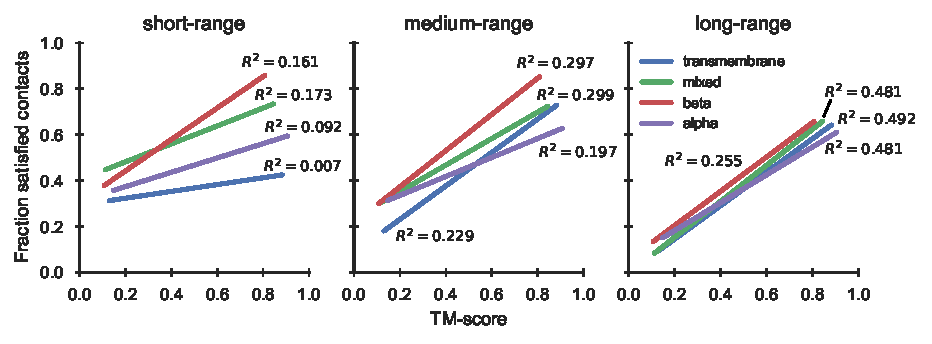
\includegraphics[width=\textwidth]{ample_decoys_smlrcstmfold.pdf}
        \caption[Linear regression model between decoy TM-score and contact satisfaction]{Linear regression model fitted to decoy TM-scores and corresponding fractions of satisfied, range-dependent contacts. Targets were further separated by fold classification. Coefficients of determination ($R^2$-values) added alongside each regression model.}
	\label{fig:ample_decoys_smlrcstmfold}
\end{figure}

An analysis of the correlation between the TM-score and long-range contact satisfaction of individual decoy sets further highlights the potential to subselect decoy sets by their long-range contact satisfaction. One hundred and eight decoy sets show statistically significant positive correlations between decoy TM-scores and their long-range contact satisfaction ($\rho$-values in range of 0.09 to 0.97 with p-value $<0.01$). A single ROSETTA decoy set, derived for the Glycolipid transfer protein with \gls{pdb} ID 2eum and restrained with METAPSICOV STAGE 1 contact data, shows a weak negative correlation ($\rho=-0.10$, $p<0.01$). The remaining four decoy sets, derived for targets with \gls{pdb} IDs 1chd, 1gm4, 2x6u and 3ouf and restrained with METAPSICOV STAGE 1 contact data except for 2x6u (PCONSC2), show no statistically significant correlation between the TM-score and long-range contact satisfaction of the decoy sets. 

A further subdivide of the previously presented data by metapredictor highlights that no predictor outperforms the others. Decoy sets calculated using predictions from all metapredictors exhibit a range of stronger to weaker correlations. Similarly, target chain length and fold do not show overall stronger or weaker correlations. 

So far, all analyses focused on entire sets of decoys (1,000 decoys per set); however, it is often desirable to know if we could better estimate the accuracy of the best decoy by some measure. \textcite{Kosciolek2014-bt} demonstrated strong positive correlations for short-, medium- and long-range contact satisfaction with a decoy's corresponding TM-score (short-range:$\rho=0.50$; medium-range:$\rho=0.57$; long-range: $\rho=0.87$). In this work, some of these findings are confirmed (short-range: no correlation; medium-range:$\rho=0.52$; long-range:$\rho=0.69$) although the strength of the correlation for long-range contact satisfaction is much weaker than previously observed (\cref{fig:ample_decoys_smlrcstmtop1}). The weak positive correlation for short-range contact satisfaction is statistically non-significant, and thus cannot be validated. 

\begin{figure}[H]
	\centering
        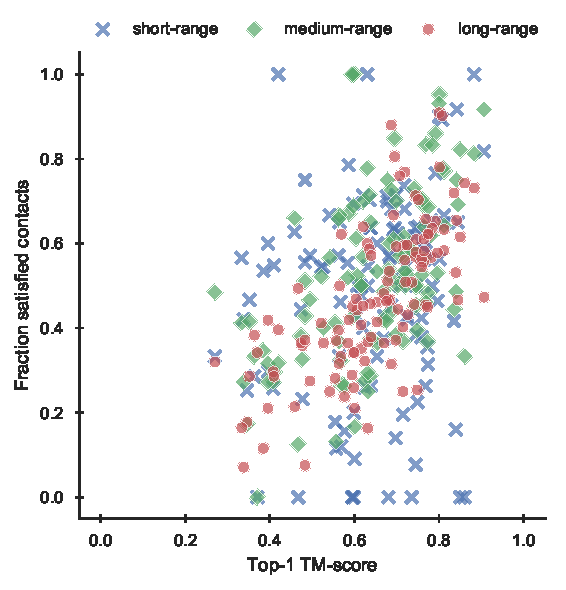
\includegraphics[width=\textwidth]{ample_decoys_smlrcstmtop1.pdf}
        \caption[Top-1 decoy TM-score and contact satisfaction analysis]{Analysis of the relationship between TM-score and contact satisfaction for the top-1 decoy (as ranked by TM-score) in each decoy set.}
	\label{fig:ample_decoys_smlrcstmtop1}
\end{figure}

\subsection{Long-range contact satisfaction metric to filter decoy sets}
In the previous section, the data highlighted that decoy quality correlates positively with contact satisfaction. In particular, a strong positive correlation between long-range contact satisfaction and decoy quality could be established for almost all decoy sets in this study. A key ambition in this work is to determine if this correlation could be used to alter the starting decoy set prior to the submission to the AMPLE cluster-and-truncate pipeline to enhance the chances of generating more successful ensemble search models for \gls{mr}.

The difference in mean TM-score of each decoy set before and after applying a subselection strategy (see \cref{sec:ample_decoys_decoy_selection}) is shown in \cref{fig:ample_decoys_deltatmsub}. Estimating a decoy's quality by short-range contact satisfaction results in marginal mean TM-score changes of decoy sets ($\Delta_{CUTOFF}=-0.003$; $\Delta_{LINEAR}=0.008$; $\Delta_{SCALED}=0.001$). In comparison, medium- ($\Delta_{CUTOFF}=0.005$; $\Delta_{LINEAR}=0.015$; $\Delta_{SCALED}=0.002$) and especially long-range ($\Delta_{CUTOFF}=0.025$; $\Delta_{LINEAR}=0.032$; $\Delta_{SCALED}=0.005$) contact satisfaction are better values to use to improve the mean TM-scores of each decoy set. Notably, per-decoy long-range contact satisfaction provides the best estimate for identifying and excluding the least accurate decoys independent of the subselection strategy. 

Given the improvement of TM-scores for each decoy set by decoy subselection, it is important to analyse the number of decoys left in each set after long-range contact-satisfaction subselection. This metric is important since too few decoys might not generate any AMPLE ensemble search models due to AMPLE's requirements after clustering and sub-clustering. For the decoy sets used in this study, the \textit{LINEAR} strategy removes on average the most decoys from each set with a fixed number of 500 (median=500). In comparison, the \textit{CUTOFF} subselection strategy removes on average 409 decoys (median=316) whilst the \textit{SCALED} method only 56 (median=29). However, the sample-dependent strategies (\textit{CUTOFF} and \textit{SCALED}) may remove a much greater number of decoys from a set if the corresponding satisfaction scores fall below a certain threshold (maximum removed by \textit{CUTOFF}=1000 and \textit{SCALED}=497). Since these numbers vary drastically similarly to the changes in TM-score, it becomes apparent that the more decoys are removed, the better the overall score becomes, which further supports the linear correlation between long-range contact satisfaction and TM-score.

In certain cases, some subselection strategies greatly altered the overall size and quality of the resulting decoy set, which started with a set of 1,000 decoys. The METAPSICOV STAGE 1 decoy set of the ankyrin sequence (\gls{pdb} ID: 2qyj) shows overall quality improvements from 0.006 (short-range \textit{SCALED}; $n_{models}=958$) to 0.213 (long-range \textit{CUTOFF}; $n_{models}=218$). The CCMPRED decoy set of sensory rhodopsin II sequence (\gls{pdb} ID: 1gu8) shows overall changes from -0.155 (short-range \textit{CUTOFF}; $n_{models}=2$) to 0.06 (long-range \textit{LINEAR}; $n_{models}=500$).

Overall, the optimal strategy to select or exclude decoys from a starting set of structures appears to be long-range contact satisfaction driving the \textit{LINEAR} strategy.

\begin{figure}[H]
	\centering
	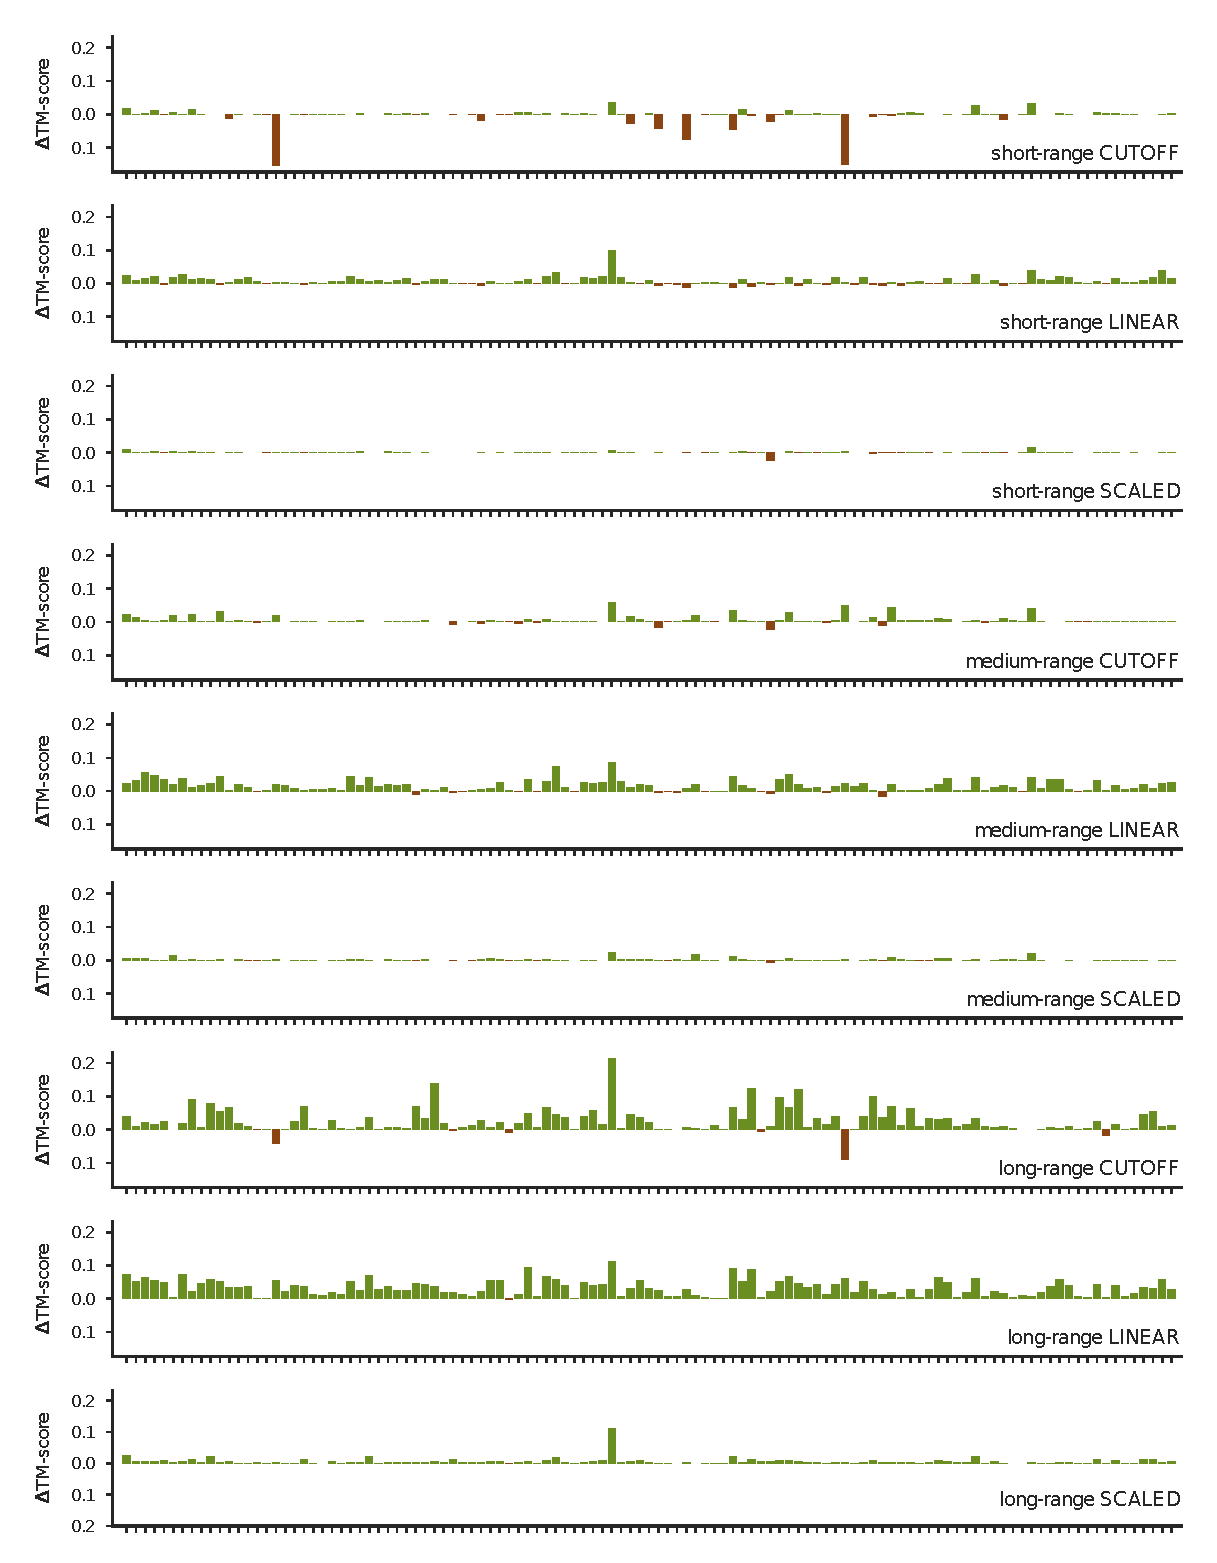
\includegraphics[width=\textwidth]{ample_decoys_deltatmsub.pdf}
        \caption[TM-score comparison pre- and post-decoy subselection]{Differences in mean TM-score  for decoy sets pre- and post-decoy subselection. Each subselection strategy is stated in each subplot along with the contact range used to establish decoy inclusion in the final set.}
	\label{fig:ample_decoys_deltatmsub}
\end{figure}

\subsection{AMPLE's cluster-and-truncate approach with filtered decoy sets}
For evaluation of performance of filtered decoy sets in \gls{mr}, a smaller sample of 35 decoy sets was selected spanning 35 unique targets (21 globular and 14 transmembrane targets). The contact prediction algorithm generating the restraints for the \textit{ab initio} structure predictions was PCONSC2 (globular targets) or CCMPRED (transmembrane targets). Each decoy set was subjected to the AMPLE pipeline with certain decoys removed according to one of four subselection strategies, namely \textit{NONE}, \textit{CUTOFF}, \textit{LINEAR} and \textit{SCALED}.

The initial step in the AMPLE pipeline is the clustering of decoys. A comparison of SPICKER clusters between the \textit{NONE} default strategy and the \textit{CUTOFF}, \textit{LINEAR} and \textit{SCALED} subselection strategies highlights an important observation. Larger clusters --- those ranked higher --- show higher similarity between a subselection strategy and the default (\cref{fig:ample_decoys_jaccluster}). The top SPICKER cluster shows high similarities between the \textit{NONE} strategy and all other subselection ones, whereby it has to be noted that the \textit{LINEAR} strategy contains only 50\% of the starting decoys and thus can at most show a Jaccard index of 0.5. With increasing cluster index, the overall similarity degrades and most of the decoys in cluster 10 are non-identical between each subselection strategy and the default. It is important to consider though that clusters might be swapped between subselection strategies, and thus the Jaccard index might not reliably indicate presence of individual decoys.

Furthermore, a similar analysis to compare the overall quality of each cluster compared to the target structure revealed less difference between the default and each subselection strategy for higher-ranked SPICKER clusters (\cref{fig:ample_decoys_tmcluster}). With decreasing SPICKER cluster index, the difference in median TM-scores starts to alternate without any particular pattern. Thus, pre-selecting decoys prior to AMPLE's cluster-and-truncate approach most certainly preserves the top cluster for the \textit{CUTOFF} and \textit{SCALED} subselection strategies, whereby lower clusters show more deviation from the default.

\begin{figure}[H]
    \centering
    \begin{subfigure}[b]{\textwidth}
        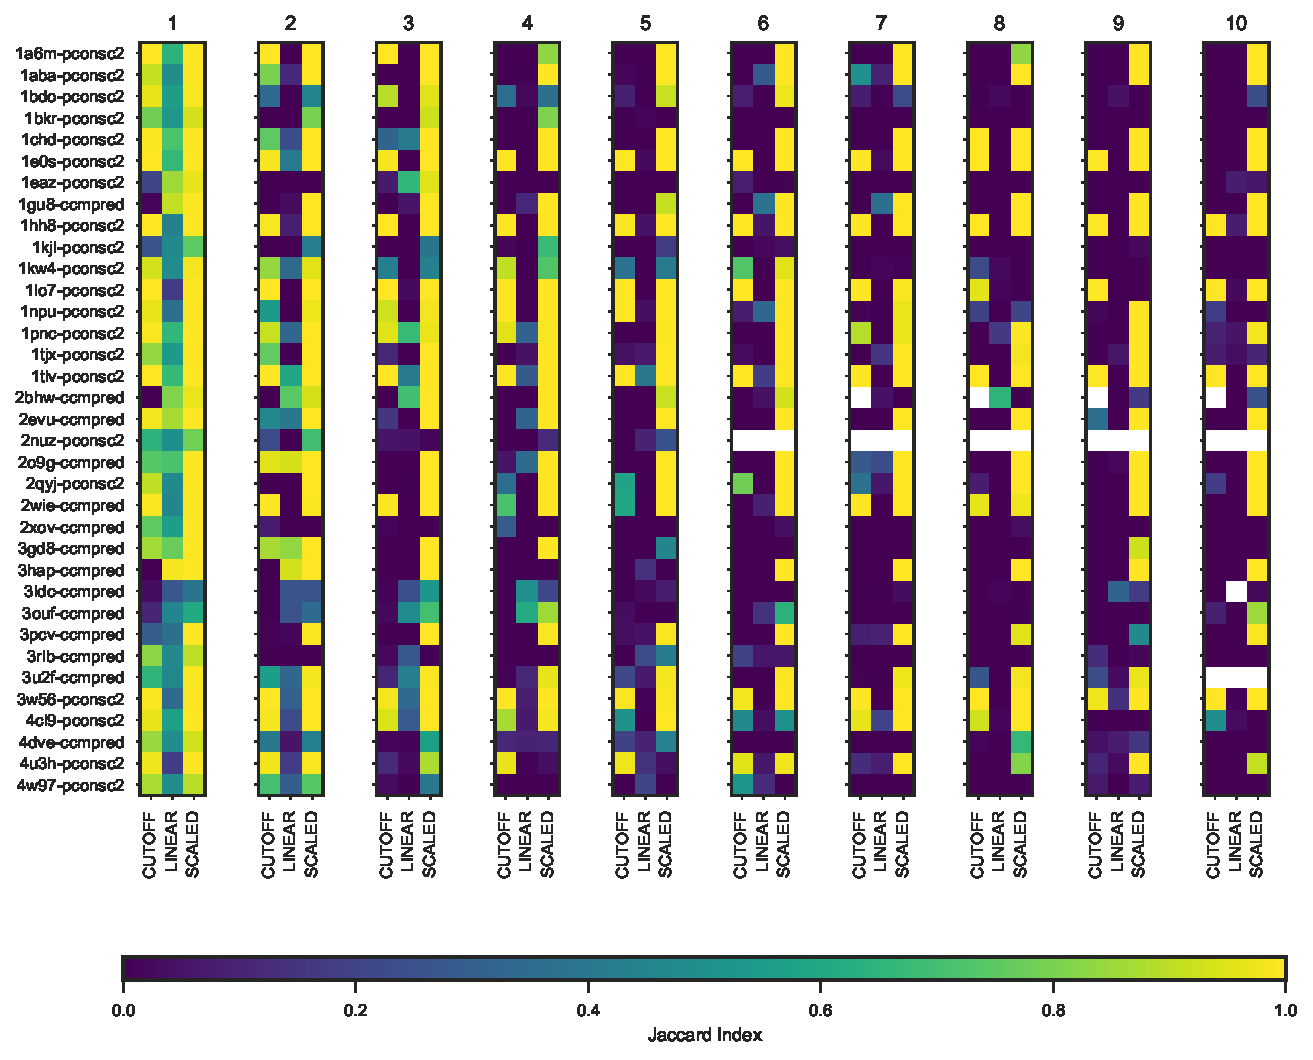
\includegraphics[width=\textwidth]{ample_decoys_jaccluster.pdf}
        \caption{}
        \label{fig:ample_decoys_jaccluster}
    \end{subfigure}
\end{figure}

\begin{figure}[H]\ContinuedFloat
    \begin{subfigure}[b]{\textwidth}
        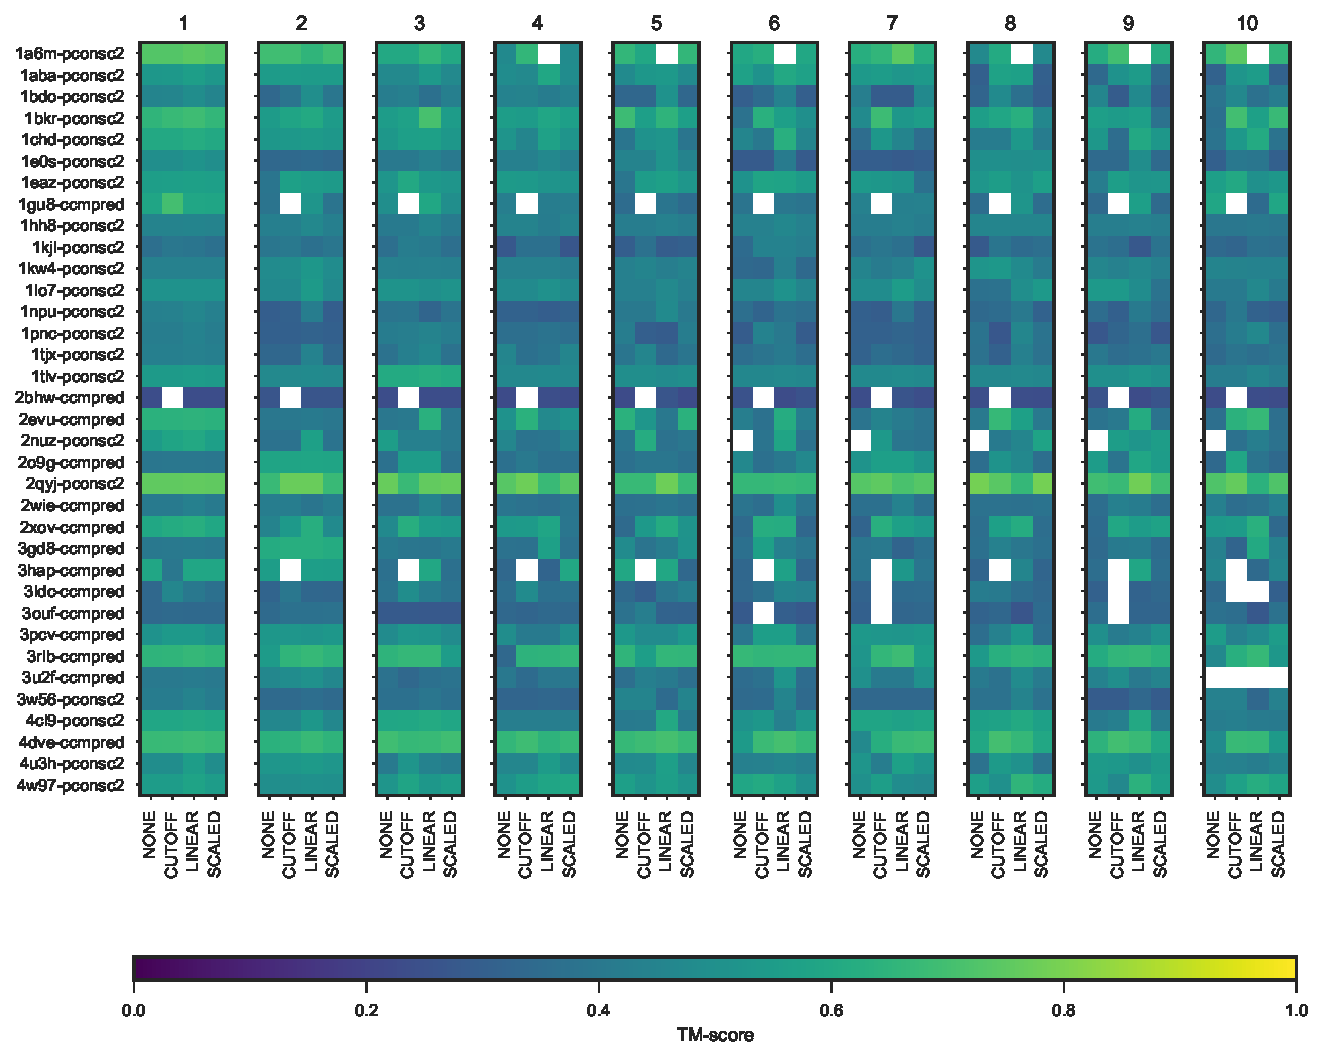
\includegraphics[width=\textwidth]{ample_decoys_tmcluster.pdf}
        \caption{}
        \label{fig:ample_decoys_tmcluster}
    \end{subfigure}
    \caption[Effect of decoy subselection on SPICKER clusters]{Effect of decoy subselection on SPICKER clusters. Effect illustrated by (a) the Jaccard Index and (b) median TM-score difference. Values were calculated for clusters resulting from the full starting set of decoys and the \textit{CUTOFF}, \textit{LINEAR} and \textit{SCALED} subselection strategies. Larger TM-score differences indicate that the subselection improved the TM-score of the cluster.}
\end{figure}

The mean of the inter-decoy variance computed by THESEUS --- used in AMPLE to guide truncation of each cluster --- is reduced in lower clusters compared to the \textit{NONE} default strategy (\cref{fig:ample_decoys_vardeltacluster}). In other words, these clusters have become more structurally homogeneous. The clusters of decoys based on the galectin-3 domain (\gls{pdb} ID: 1kjl) sequence show overall the highest reduction in mean inter-decoy variance up to -15\AA\textsuperscript{2} compared to the default strategy. Similarly, clusters 4 and 8 of the K\textsuperscript{+}-channel protein domain (\gls{pdb} ID: 3ouf) show reductions in mean inter-decoy variance of up to -20\AA\textsuperscript{2}. In general, clusters starting from \textit{CUTOFF}-subselected decoys show the greatest mean inter-decoy variance reductions, followed by \textit{LINEAR} and then \textit{SCALED}-subselected decoys sets.

\begin{figure}[H]
    \centering
    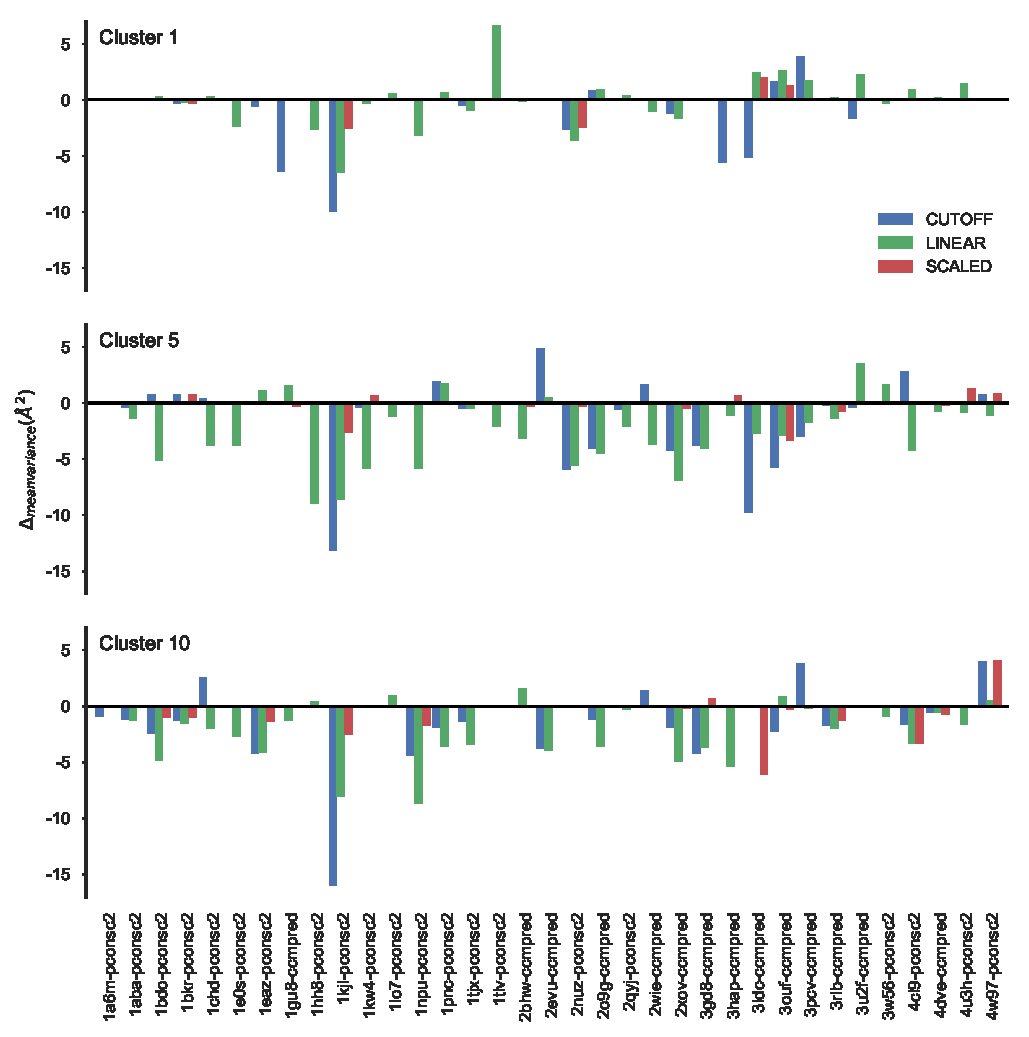
\includegraphics[width=\textwidth]{ample_decoys_vardeltacluster.pdf}
    \caption[Effect of decoy subselection on THESEUS variance]{Effect of decoy subselection on mean inter-decoy THESEUS variance. Difference in mean variance calculated between the default and the three decoy subselection strategies \textit{CUTOFF}, \textit{LINEAR} and \textit{SCALED}. Data for clusters 1, 5 and 10 shown as examples.}
    \label{fig:ample_decoys_vardeltacluster}
\end{figure}

A comparisons of intermediate stages in the AMPLE pipeline resulting from differently subselected decoy sets is very difficult. Each strategy results in different starting sets, which result in different clusters. Since AMPLE's objective truncation procedure is based on the inter-decoy variance, it might be greatly affected by differing clusters. Nevertheless, structure solution is more likely when AMPLE generates more ensemble search models because a greater number of search models flects greater inter-cluster decoy similarity and trialling a greater number should provide a higher chance of success. A count of generated AMPLE ensemble search models reveals that the \textit{SCALED} strategy generates the most search models ($n=7,611$), which is roughly 300 more than the default \textit{NONE} strategy ($n=7,340$). The \textit{CUTOFF} subselection strategy generates the least ensemble search models ($n=7,237$), whilst the \textit{LINEAR} strategy's count ($n=7,401$) is very similar to the \textit{NONE} one.

Further inspection of the number of AMPLE-generated ensemble search models by target reveal near identical numbers between the \textit{NONE}, \textit{LINEAR} and \textit{SCALED} strategies (\cref{fig:ample_decoys_mrsuccesstarget}). In fact, only a few outliers for each of those methods distinguish them from the others. The \textit{CUTOFF} strategy shows greater deviation from the other three, especially for certain targets with differences up to approximately 200 ensemble search models (\cref{fig:ample_decoys_mrsuccesstarget}). If we compare all these strategies to the previous default processing in AMPLE (\textit{NONE\_classic}; further details in \cref{subsec:ample_decoys_methods_mr}), we can see that the number of search models is greatly reduced (\cref{fig:ample_decoys_mrsuccesstarget}). A comparison of the previous default (\textit{NONE\_classic}) with the new one (\textit{NONE}) shows on average 144 fewer ensemble search models per target, whilst sampling a larger range of folds through all 10 clusters.

\subsection{MR search models by processing single decoys}
In addition to the decoy set subselection, this study also attempts to identify single decoys of sufficient quality to be used directly as \gls{mr} search models. Although ensembles are generally more desirable \gls{mr} search models \cite{Rigden2018-zt,Keegan2018-kn,Thomas2015-wu}, individual decoys might be successful by themselves, and thus save the overhead of generating and trialling a great number of AMPLE ensemble search models. Thus, the top-5 decoys, as judged by long-range contact satisfaction, were selected from each decoy set. Four distinct processing approaches were applied to each decoy to eliminate less reliable parts, and subsequently compared against the unmodified initial decoy.

The correlation between a decoy's long-range contact satisfaction and its TM-score has previously been outlined and is further confirmed here (\cref{fig:ample_decoys_individualinitial}). However, the positive correlation was dependent on the target's fold class and the overall accuracy of the decoy set. Here, an analysis of the top-5 decoys by long-range contact satisfaction in each decoy set shows that 50\% of selected decoys fall in the 80\textsuperscript{th} percentile or greater of TM-scores in each decoy set whilst 90\% are in the at least the 40\textsuperscript{th} percentile (\cref{fig:ample_decoys_individualinitial}). 

\begin{figure}[H]
	\centering
	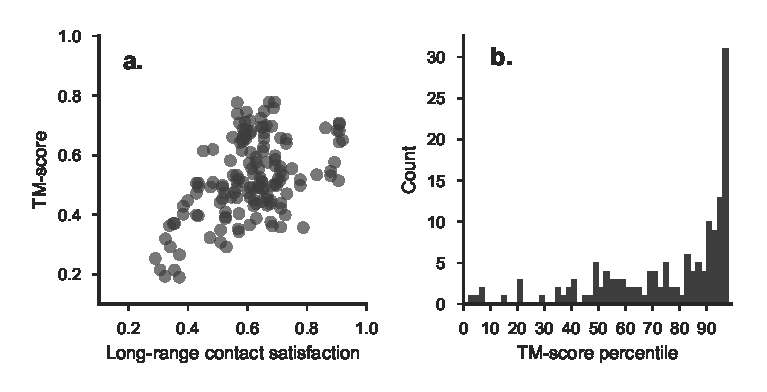
\includegraphics[width=\textwidth]{ample_decoys_individualinitial.pdf}
        \caption[Selection of single decoys by long-range satisfaction]{Analysis of long-range contact-satisfaction-based decoys with respect to the relationship between (a) the satisfaction and decoy quality and (b) the quality compared to the remaining, excluded decoy set.}
	\label{fig:ample_decoys_individualinitial}
\end{figure}

A comparison of \gls{rmsd} value changes indicated that the ``fragment'' and ``variance'' metrics provide the best approximation to identifying less-reliable regions in each decoy. The average \gls{rmsd} change compared to the original decoys is just under 4.0\AA. This compares to a slightly lower \gls{rmsd} change of 2.1\AA\ for ``DSSP''-treated decoys and 1.5\AA\ for the ``domain'' treatment. Although almost all decoys were improved by either of the treatments, a small number of decoys worsen in terms of \gls{rmsd} compared to its native structure. All treatments except the ``fragment'' one had worsened decoys in the final set, with changes up to -1.6\AA. 

A comparison of the range of \gls{rmsd} values revealed much greater changes for the ``fragment'' and ``variance'' conditions (\cref{fig:ample_decoys_individualrmsd}). However, these changes are not reflected in the fraction of residues retained in each decoy. Most residues were removed by the ``domain'' treatment (\textmu=61.6\%), whilst the ``fragment'' one saw the least removal (\textmu=34.5\%). Similarly to the range in \gls{rmsd} values, the ``fragment'' and ``variance'' treatments resulted in the greatest spread of fraction of residues in the treated decoy. The values range for both treatments from retaining less than 5\% of the initial decoy up to 100\%.

\begin{figure}[H]
	\centering
	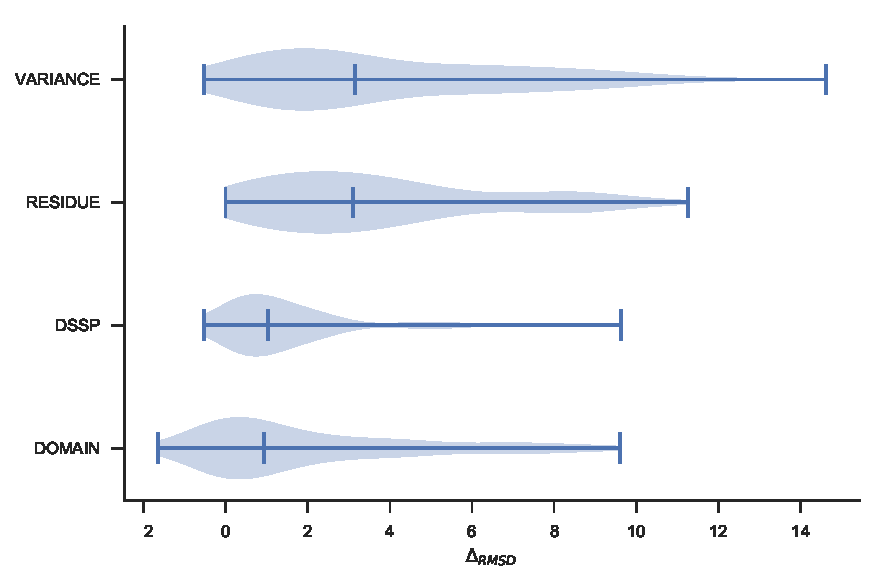
\includegraphics[width=\textwidth]{ample_decoys_individualrmsd.pdf}
        \caption[Difference in RMSD for individually processed decoys]{Distribution of differences in \gls{rmsd} values between the initial and modified decoys under four different treatments. A positive \textDelta\textsubscript{RMSD} value corresponds to a decrease in \gls{rmsd} compared to the crystal structure.}
	\label{fig:ample_decoys_individualrmsd}
\end{figure}

A further aspect of the decoy treatments highlights that the fraction of residues retained after decoy post-processing correlates with the cluster variance of the decoy, extracted from THESEUS results of each decoy's cluster in the \textit{NONE} strategy (\cref{fig:ample_decoys_individualcorrtm}). Unlike the variance metric, all other processing metrics do not show a correlation with the fraction of residues retained. This explains at least in part why we see much greater changes in \gls{rmsd} value between the initial and processed decoy for the ``variance'' treatment compared to the others. However, if a decoy is of particularly poor quality (TM-score $<0.3$), the ``variance'' treatment retains as little as 0.87\% and 1.7\% of the initial decoy (2 and 4 residues) whilst the others retain a much larger fraction of at least 40\% for equivalent decoys.

\begin{figure}[H]
        \centering
        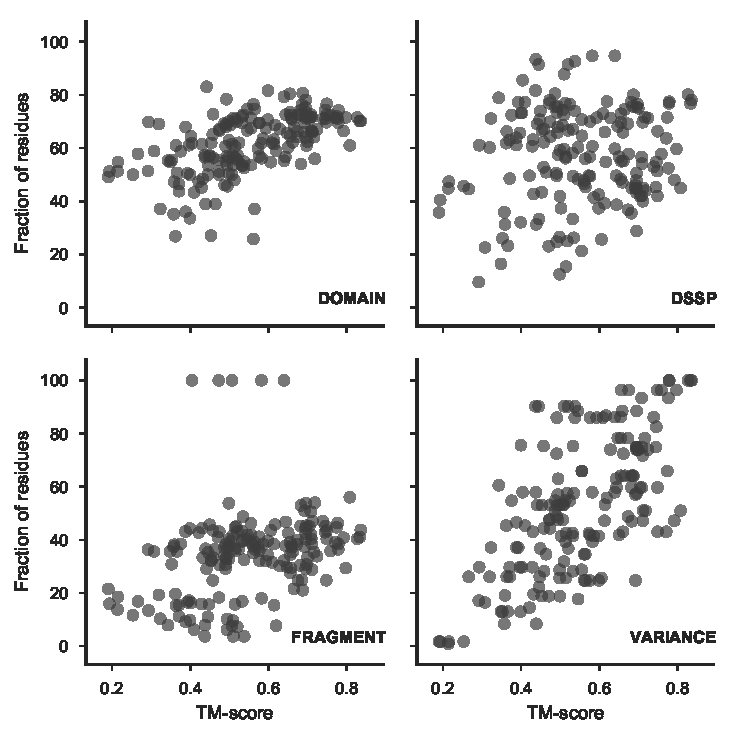
\includegraphics[width=\textwidth]{ample_decoys_individualcorrtm.pdf}
        \caption[Relationship between decoy quality and fraction of residues retained]{Scatter plots of initial decoy TM-score and the fraction of residues retained after one of four different residue removal treatments.}
        \label{fig:ample_decoys_individualcorrtm}
\end{figure}

\subsection{Decoy subselection extends AMPLE's performance}
The final step in this study is the assessment of AMPLE-generate ensemble search models and single-decoy-based search models in \gls{mr}. In particular, the comparison of different decoy subselection strategies and individual decoy-processing treatments is of great interest since it might allow us to extend AMPLE's performance beyond that described in previous chapters.

A comparison of the total number of targets solved by each subselection strategy shows that the \textit{CUTOFF}-subselected decoys lead to most structure solutions (14 out of 35) (\cref{fig:ample_decoys_mrsuccesstarget}). Although slightly less successful, the \textit{LINEAR} and \textit{SCALED} subselection strategies lead to structure solutions of two additional targets compared to the \textit{NONE} strategy (11 out of 35). The \textit{LINEAR} and \textit{SCALED} strategies are on par with AMPLE's default, the \textit{NONE\_classic} strategy (\cref{fig:ample_decoys_mrsuccesstarget}). Although the \textit{NONE\_classic} strategy generates two version of each ensemble search model with poly-Alanine and all-atom side chain treatment, the former was enough to solve all targets outlined in (\cref{fig:ample_decoys_mrsuccesstarget}). Therefore, the \textit{LINEAR} and \textit{SCALED} subselection strategies would be the minimum processing requirement to solve the same number of targets with fewer search models and hence improved performance.

\begin{figure}[H]
    \centering
    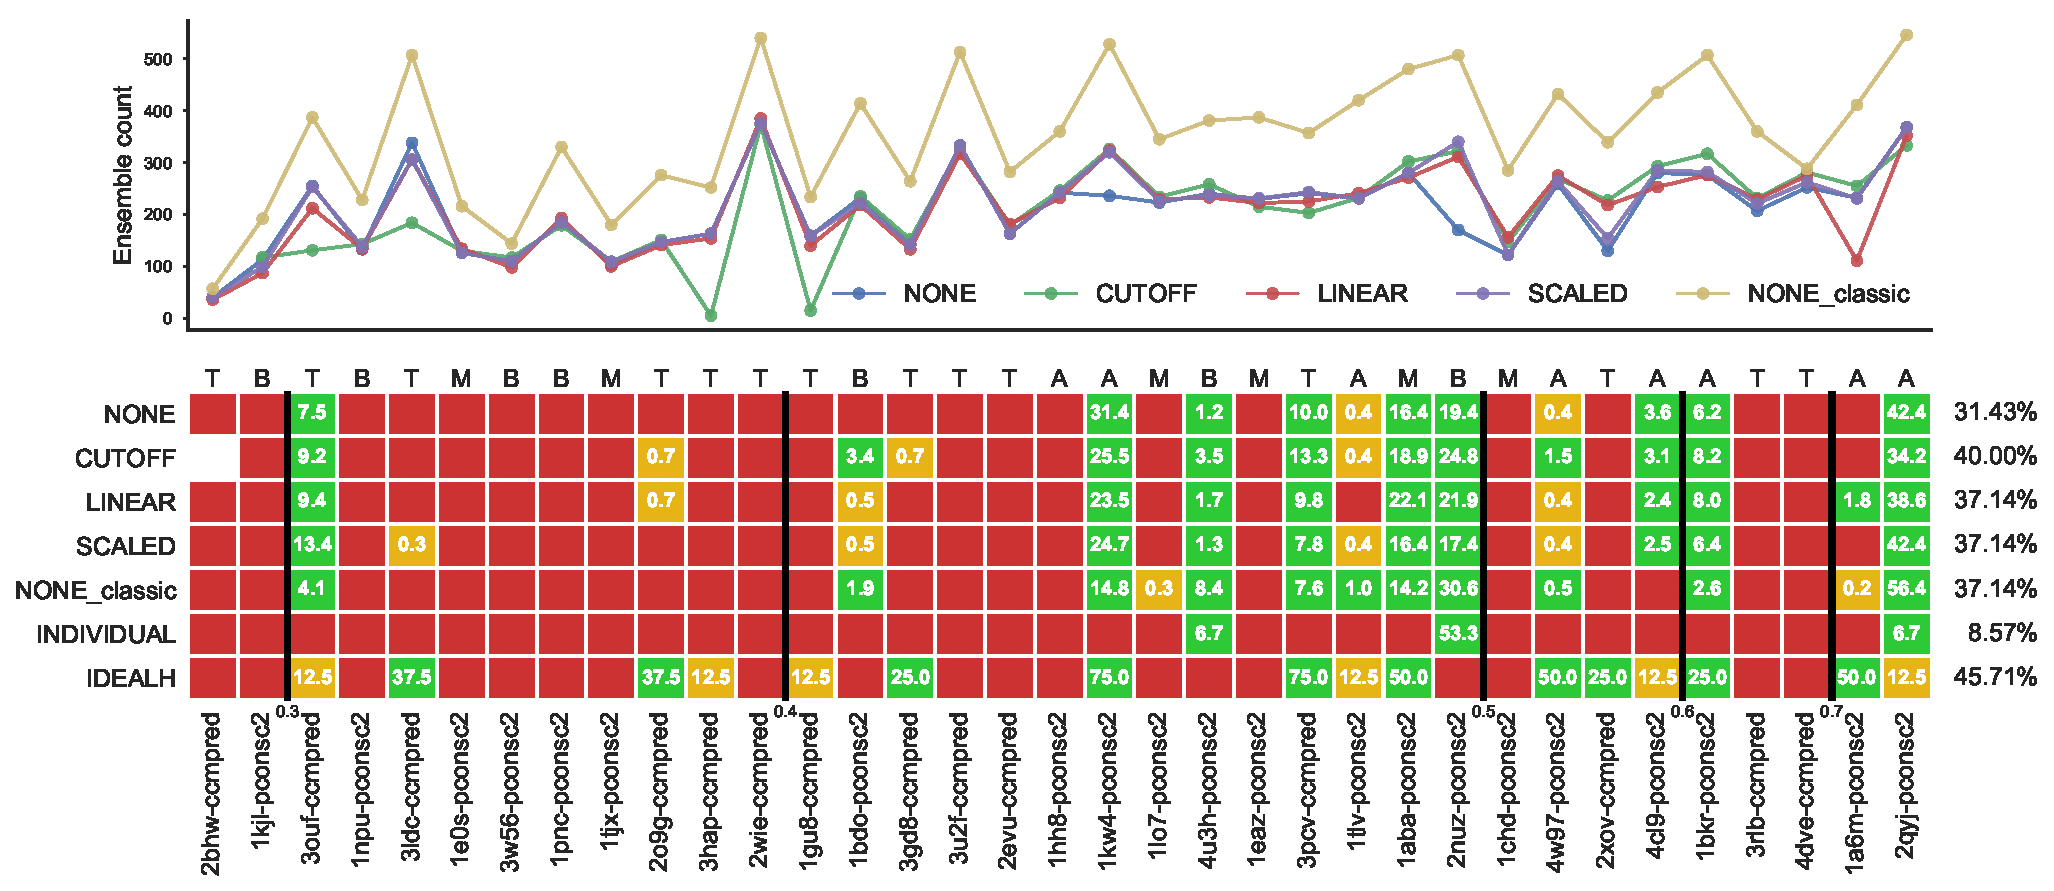
\includegraphics[width=\textwidth]{ample_decoys_mrsuccesstarget.pdf}
\caption[Molecular Replacement summary of decoy-subselected AMPLE ensembles]{Molecular Replacement summary of decoy-subselected AMPLE ensembles. AMPLE-generated ensemble counts illustrated at the top with Molecular Replacement results in grid below: red cell equates to no solution; orange to a singleton solution; and green to multiple solutions. All \textit{INDIVIDUAL} attempts were compressed to a single row per decoy set. The number in the orange and green cells indicates the percentage of ensemble search models leading to structure solutions. One letter code above each column indicates the target fold: ``T'' for transmembrane; ``A'' for all-\textalpha; ``B'' for all=\textbeta; ``M'' for mixed \textalpha-\textbeta. Values alongside each row indicate the number of targets with structure solutions and total number targets attempted. Targets are sorted from left to right with increasing median TM-score of the starting decoy set. The black lines highlight TM-score thresholds from 0.3 to 0.7 from left to right. The subselection strategy \textit{IDEALH} refers AMPLE's ideal helix library.}
    \label{fig:ample_decoys_mrsuccesstarget}
\end{figure}

The \textit{CUTOFF} method yields the highest number of structure solutions based on AMPLE-generated ensemble search models whilst generating the fewest search models. In fact, this subselection strategy has generated no ensemble search models for target 2bhw. Furthermore, the \textit{CUTOFF} method achieves amongst the best ratio of search models leading to structure solution compared to the total number generated. 

In a few cases, only a single AMPLE search model led to a structure solution (orange cells in \cref{fig:ample_decoys_mrsuccesstarget}). Upon closer inspection, 71\% of all singleton solutions were achieved with AMPLE ensemble search models containing at least 30\% of the target sequence. Twenty-nine percent of the singleton solutions contain at least 50\% of the target sequence, whilst none contain more than 70\%. Three out of four search models with less than 30\% of the target sequence were derived from the PCONSC2 decoy set predicted for the ketosteroid transcriptional regulator KstR2 (\gls{pdb} ID: 4w97) sequence and contained one, two or three small helical fragments.  

In certain cases the subselection of starting decoys made a subtle yet essential difference to generate an AMPLE ensemble search model for successful structure solution. An example of such a case is the CCMPRED decoy set of the aquaporin Z domain with \gls{pdb} ID 2o9g. \textit{CUTOFF} and \textit{LINEAR} subselected decoys led to a single search model each (cluster 1; 59\% truncation and subclustering radius of 3\AA), which was sufficient for structure solution (\cref{fig:ample_decoys_mrsuccesstarget}). The \textit{NONE} and \textit{SCALED} subselection strategies generated the same ensemble, which did not lead to structure solution (\cref{fig:ample_decoys_mrsuccesstarget}). An analysis of the decoys in the ensembles reveals that 30\% (9 out of 30) are different between the successful ensembles and the \textit{NONE} strategy. However, only a single decoy is unique to either \textit{CUTOFF} and \textit{LINEAR} in a direct comparison. Ultimately, this results in a \gls{rmsd} difference between the \textit{NONE} and \textit{CUTOFF} ensembles of 2.25\AA\ (\cref{fig:ample_decoys_2o9g_example}), whilst the \textit{CUTOFF} and \textit{LINEAR} ensembles are identical (\gls{rmsd}=0.00\AA). Thus, subselection shows crucial value in preparing decoy datasets prior to AMPLE's cluster-and-truncate approach.

\begin{figure}[H]
    \centering
    \includegraphics[width=\textwidth]{ample_decoys_2o9g_example.pdf}
    \caption[Comparison of ensembles derived from differently subselected decoys]{Example of the structural divergence of two ensemble search models with an identical AMPLE cluster-and-truncate path. Ensembles are based on the CCMPRED decoy set of \gls{pdb} ID 2o9g and derived from cluster 1 with 59\% truncation and subclustering radius of 3\AA. The blue ensemble was derived from \textit{CUTOFF} subselected decoys and the red ensemble without subselection. The blue ensemble search model is successful in deriving a \gls{mr} structure solution, the red one is not. The arrow indicates the substructure with the highest degree of structural divergence.}
    \label{fig:ample_decoys_2o9g_example}
\end{figure}

The rank order of targets by median TM-score of the initial starting decoy set in \cref{fig:ample_decoys_mrsuccesstarget} shows that no decoy set with median TM-score of less than 0.3 score units led to structure solution; however, only two such cases exist in the dataset, and therefore this threshold may only serve as indication. With increasing median TM-score, i.e. increasing similarity between the decoy set and its reference target structure, the chances appear to increase to achieve structure solution. Beyond a threshold of 0.4 TM-score units, structure solutions are much more likely (over 50\% of targets solved with one of the four subselection strategies), which highlights AMPLE's success in processing such accurate decoy sets appropriately.

The work in this study further explored whether individual decoys could be selected via their long-range contact satisfaction and trialled directly as \gls{mr} search models. The \textit{INDIVIDUAL} subselection strategy explored this aspect with a variety of post-selection processing approaches. However, structure solutions for only three targets could be obtained using this single-decoy approach (\cref{fig:ample_decoys_mrsuccesstarget}). All processing strategies obtained lead to structure solutions based on the PCONSC2 decoy set of the \textalpha-spectrin SH3 domain (\gls{pdb} ID: 2nuz). The other two targets with solutions, \gls{pdb} IDs 2qyj and 4u3h with PCONSC2 decoy sets, solved at least once with a single decoy subjected to the ``domain'', ``DSSP'', ``fragment'' or ``variance'' treatments. Across the three targets, only five decoys (three based on the sequence of \gls{pdb} ID 2nuz) with a minimum TM-score of 0.682 resulted in the 20 structure solutions (\gls{pdb} ID 2nuz: 16 solutions; \gls{pdb} ID 2qyj: 2 solutions; \gls{pdb} ID 4u3h: 2 solutions).

A comparison of decoy-derived search models and AMPLE's simplistic ideal helix library \cite{Thomas2015-wu} in \gls{mr} was done. Ideal helices achieved the most structure solutions solving 16 out of 35 targets (\cref{fig:ample_decoys_mrsuccesstarget}). In particular, ideal helices achieved structure solutions for more transmembrane targets. Eight out of 14 transmembrane targets were solved with at least one ideal helix, which compares to six out of 14 for all decoy-based search models combined. No transmembrane target was solved with decoy-based search models that could not be solved with ideal helices. The number of solved transmembrane targets is also increased by two compared to the work by \textcite{Thomas2017-sh}, which is due to improved \gls{mr} software. Ideal helices also managed to achieve near identical results for all-\textalpha\ and mixed \textalpha-\textbeta\ targets in the set compared to decoy-derived search models. However, four targets remained intractable by ideal helices yet were solved with decoy-based search models. Three of these targets are all-\textbeta\ targets (\gls{pdb} IDs: 1bdo, 2nuz and 4u3h) and the fourth a mixed \textalpha+\textbeta\ one (\gls{pdb} ID: 1lo7). Lastly, \textcite{Thomas2017-sh} suggested that decoy-derived search models are essential since ideal helices provide insufficient scattering matter with low resolution ($>2$\AA) intensity data. In this study, these findings cannot be validated given that \gls{pdb} ID 1gu8 (resolution of 2.27\AA) was solved solely with ideal helices whilst being the target with the lowest resolution of all solved ones.

\section{Discussion}
The subselection of decoy sets by long-range contact satisfaction is a concept originally proposed by \textcite{Kosciolek2014-bt} and later confirmed and extended by \textcite{De_Oliveira2017-gj} and \textcite{Adhikari2018-lj}. In this study, these findings are further confirmed by re-analysing all decoy sets previously presented in this thesis. 

Furthermore, the benefit of subselecting decoys based on their long-range contact satisfaction pre-AMPLE was evaluated. Subselection extends the target tractability of AMPLE whilst reducing the number of generated search models, which effectively enhances AMPLE's performance. The \textit{CUTOFF} subselection strategy has proven to be most successful in flagging the worst decoys, which results in more accurate ensemble search models being generated. The data presented shows that subtle differences in clustering can have significant effects on ensemble search model generation resulting in the loss or gain of structure solutions. Finally, given that the \textit{NONE} strategy has become AMPLE's default since this study was conducted, the results are important for AMPLE users to improve the chances of structure solution. 

Based on the results in this work it has also become apparent that decoy-based ensemble search models are inferior to AMPLE's simple ideal helix library, particularly for transmembrane protein targets. The latter is sufficient to solve the majority of transmembrane protein targets, which outperforms all decoy-based approaches combined. This result constradicts the one reported by \textcite{Thomas2017-sh}, who found that decoy-based search models are required when the resolution was worse than 2\AA. Furthermore, it is expected that the application of more sophisticated ideal helix library approaches, such as ARCIMBOLDO \cite{Millan2015-uf} or FRAGON \cite{Jenkins2018-gf}, will make decoy-based search models less needed for transmembrane targets. However, decoy-based search models are still required, especially for globular folds with little or no helical secondary structure. Decoy-based search models are also needed when the resolution of the experimental data is low ($<2$\AA). In such cases, \gls{mr} algorithms require higher proportions of scattering matter compared to the asymmetric unit content to detect the signal of a correctly placed search model \cite{McCoy2017-cz}. Since it is easier to derive larger search models by truncating sequence-specific decoys than identifying larger fragments or even substructures, decoy-based search models are still needed.

Beyond subselecting decoys sets, some very preliminary work in this chapter aimed to explore the possibility of identifying, processing and trialling individual \textit{ab initio} structure predictions as \gls{mr} search models. Although previous work has extensively demonstrated the benefits of ensembles over individual search models in \gls{mr} \cite{Rigden2018-zt,Keegan2018-kn,Thomas2015-wu}, interest in this approach remains. In particular, individual decoys with high similarity to the crystal structure are sometimes present amongst 1,000 non-native-like starting decoys. Although such decoys are included in AMPLE ensemble search models, trialling them individually might enhance the performance of AMPLE by avoiding the generation and trial of potentially hundreds of ensemble search models. As such, identification and \gls{mr} trial could be crucial to solving a target, whose sequence was used to predict the decoys. However, findings in this work supported previous challenges in the field of identifying the very best decoys reliably by long-range contact satisfaction \cite{Adhikari2018-lj,De_Oliveira2017-gj,Kosciolek2014-bt}. Although a general correlation exists for most decoy sets, the best decoy by long-range contact satisfaction is not necessarily the very best by TM-score. Thus, the data suggests that AMPLE's ensembling approach remains the more successful. Nevertheless, further work needs to be conducted to explore alternate decoy processing options. These could include a combination of metrics used in this study, or alternatives such as solvent accessible surface. Furthermore, exploiting contact information to aid AMPLE's cluster-and-truncate approach could prove a promising alternative, too.
